%=======================================================
% CHAPTER 4: CRYPTOGRAPHIC LATTICES
%=======================================================

\begin{frame}[plain]
  \begin{center}\bfseries\centering
    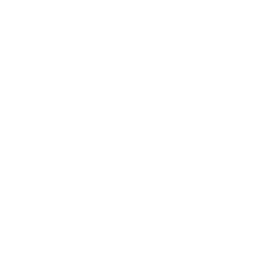
\includegraphics[scale=1]{assets/branding/opa0}
    \vspace{-5.75cm}\\
    {\adjustbox{scale=1.65}{\color{TealDarkCyan}\;V.\;Cryptographic Lattices}}
    \vspace{.25cm}
    \begin{minipage}{.78\textwidth}
      \scriptsize\color{Ink}
      \textbf{Big picture.}\; LWE/LWR are noisy decoding templates; SIS is a short-relation template.\\[.2cm]
      \textbf{Details to watch.}\; $q$-ary lattices, rings, modules, rounding, parameters, and reductions.
    \end{minipage}
    {\ }\vspace{2.1cm}\\
    \bigskip
  \end{center}
\end{frame}

\begin{frame}[shrink=10]{\textbf{V. Cryptographic Lattices}}{$q$-ary Lattices}
\defbox[$q$-ary lattice from a matrix]{
Let $\mat A\in\Z_q^{m\times n}$. Define
\[
  \Lambda_q^\perp(\mat A)
  =\set{x\in\Z^n:\mat A x\equiv 0\pmod q}.
\]
This is an integer lattice containing $q\Z^n$.
}
\begin{itemize}
  \item Modular linear algebra becomes lattice geometry after lifting to $\Z^n$.
  \item The determinant is typically a power of $q$ when $\mat A$ has full rank modulo $q$.
  \item Short integer relations modulo $q$ are short lattice vectors.
\end{itemize}
\textbf{Toy example.}\; Take $q=5$ and $\mat A=[1\ \ 2]$.
Then
\[
  \Lambda_5^\perp(\mat A)=\set{(x_1,x_2)\in\Z^2:x_1+2x_2\equiv0\pmod5}.
\]
The vector $(3,1)$ lies in this lattice because $3+2=5$.
\vspace{-.1cm}
\begin{center}
\begin{tikzpicture}
  \node[process] (mod) {modular equations\\[-1pt]$\mat A x=0\bmod q$};
  \node[process blue, right=1.4cm of mod] (lat) {integer lattice\\[-1pt]$x\in\Lambda_q^\perp(\mat A)$};
  \node[process amber, right=1.4cm of lat] (short) {short relation\\[-1pt]$\norm{x}$ small};
  \draw[flow] (mod) -- (lat);
  \draw[flow blue] (lat) -- (short);
\end{tikzpicture}
\end{center}
\end{frame}

\begin{frame}[shrink=8]{\textbf{V. Cryptographic Lattices}}{Problem Family Map}
\begin{center}
\renewcommand{\arraystretch}{1.22}
\begin{tabular}{p{.19\textwidth}p{.30\textwidth}p{.39\textwidth}}
\toprule
Problem & Public data & Hidden object \\
\midrule
LWE & noisy linear equations over $\Z_q$ & secret $s$ or non-randomness \\
Ring-LWE & noisy equations over $R_q=\Z_q[x]/(f)$ & polynomial secret $s$ \\
Module-LWE & noisy equations over $R_q^k$ & vector of polynomial secrets \\
LWR & rounded linear equations & rounding error replaces sampled noise \\
SIS & matrix $\mat A$ over $\Z_q$ & short relation $x$ with $\mat A x=0$ \\
Module-SIS & matrix over $R_q$ & short module relation \\
\bottomrule
\end{tabular}
\end{center}
\vspace{-.1cm}
\textbf{Two recurring templates.}
\[
  \text{LWE side: noisy or rounded equations}
  \qquad
  \text{SIS side: short modular relations.}
\]
\textbf{Why so many names?}\; Plain matrix problems are conceptually clean.
Ring and module versions add algebraic structure for compact keys and fast arithmetic while trying to preserve lattice hardness.
\end{frame}

\begin{frame}[shrink=6]{\textbf{V. Cryptographic Lattices}}{The Common Hardness Pattern}
\small
\begin{center}
\renewcommand{\arraystretch}{1.20}
\begin{tabular}{>{\bfseries}p{.22\textwidth}p{.31\textwidth}p{.33\textwidth}}
\toprule
Lens & LWE/LWR side & SIS side \\
\midrule
Public object & samples $(\mat A,b)$ & matrix or module map $\mat A$ \\
Hidden witness & secret $s$ and small error & nonzero short relation $x$ \\
Verification & decode or distinguish & check $\mat A x=0\bmod q$ and $\norm{x}\le\beta$ \\
Geometry & BDD / closest point & SVP-like short-vector search \\
Structured forms & rings and modules compress $\mat A$ & rings and modules compress relations \\
\bottomrule
\end{tabular}
\end{center}
\vspace{-.1cm}
\thmbox[One template, many interfaces]{
The details change from vectors to polynomials to modules, but the hard step is always geometric:
recover the small object hidden inside a modular algebraic description.
}
\end{frame}

\begin{frame}[shrink=5]{\textbf{V. Cryptographic Lattices}}{SIS}
\defbox[Short Integer Solution]{
Given a random matrix $\mat A\in\Z_q^{m\times n}$, find a nonzero short vector $x\in\Z^n$ such that
\[
  \mat A x\equiv 0\pmod q.
\]
}
\begin{columns}[T,onlytextwidth]
\begin{column}{.48\textwidth}
\textcolor{TealDarkCyan}{\textbf{Lattice form}}
\[
  x\in\Lambda_q^\perp(\mat A),\qquad 0<\norm{x}\le \beta.
\]
SIS is a short-vector problem in a $q$-ary lattice.
\textbf{Toy relation.}\; For $\mat A=[1\ \ 2]\bmod5$, $x=(3,1)$ satisfies $\mat A x=5\equiv0$.
Real SIS uses dimensions where finding such short relations is hard.
\end{column}
\begin{column}{.48\textwidth}
\textcolor{TealDarkCyan}{\textbf{Cryptographic intuition}}
\begin{itemize}
  \item Easy to verify: compute $\mat A x\bmod q$.
  \item Hard to find when parameters make short relations rare.
  \item Gives collision-resistant hashing and signatures.
\end{itemize}
\end{column}
\end{columns}
\end{frame}

\begin{frame}{\textbf{V. Cryptographic Lattices}}{Visualization: SIS as Congruence Lines}
\small
\begin{columns}[T,onlytextwidth]
\begin{column}{.50\textwidth}
\textbf{Toy kernel.}\; For $q=5$ and $\mat A=[1\ \ 2]$,
\[
  x_1+2x_2\equiv0\pmod5.
\]
The lattice is the union of integer points on the parallel lines
\[
  x_1+2x_2=5k,\qquad k\in\Z.
\]
\textbf{SIS asks for a short nonzero point on these lines.}
\end{column}
\begin{column}{.46\textwidth}
\begin{center}
\begin{tikzpicture}[scale=.43,transform shape]
  \useasboundingbox (-5.3,-5.55) rectangle (5.3,4.4);
  \draw[panel] (-5.3,-4.4) rectangle (5.3,4.4);
  \begin{scope}
  \clip (-5.3,-4.4) rectangle (5.3,4.4);
  \foreach \x in {-5,...,5}{
    \draw[thin lattice line] (\x,-4.1) -- (\x,4.1);
  }
  \foreach \y in {-4,...,4}{
    \draw[thin lattice line] (-5.1,\y) -- (5.1,\y);
  }
  \foreach \k in {-2,...,2}{
    \draw[BlueCode!32,line width=.9pt] (-5,{(5*\k+5)/2}) -- (5,{(5*\k-5)/2});
  }
  \foreach \x in {-5,...,5}{
    \foreach \y in {-4,...,4}{
      \node[circle,fill=Ink!35,inner sep=.8pt] at (\x,\y) {};
    }
  }
  \foreach \x/\y in {0/0,3/1,1/2,-2/1,-4/2,2/-1,4/-2,-1/-2,-3/-1}{
    \node[circle,fill=ErrorRed,inner sep=2.0pt] at (\x,\y) {};
  }
  \draw[short vector] (0,0) -- (3,1) node[above right] {$(3,1)$};
  \end{scope}
  \node[caption text,align=center,text width=5.5cm] at (0,-5.05)
    {red points satisfy $x_1+2x_2\equiv0\bmod 5$};
\end{tikzpicture}
\end{center}
\end{column}
\end{columns}
\end{frame}

\begin{frame}[shrink=8]{\textbf{V. Cryptographic Lattices}}{LWE}
\defbox[Learning With Errors]{
Let $s\in\Z_q^n$ be secret. Given samples
\[
  (a_i,\ b_i=\inner{a_i}{s}+e_i \bmod q),
\]
where $a_i\leftarrow\Z_q^n$ and $e_i$ is small, recover $s$ or distinguish the samples from uniform.
}
\begin{itemize}
  \item Without error, this is linear algebra over $\Z_q$.
  \item With small error, the equations are only approximately consistent.
  \item The error hides the exact lattice hyperplanes that would reveal $s$.
\end{itemize}
\bigskip
\textbf{\color{red}Core idea.}\; Noise turns an easy algebra problem into a closest-vector style problem.
\textbf{One sample.}\; Let $q=17$, $a=(3,5)$, $s=(4,2)$, and $e=-1$.
Then
\[
  b=\inner{a}{s}+e=3\cdot4+5\cdot2-1=21\equiv4\pmod{17}.
\]
Without the error, the value would be $5$; the small shift hides the exact equation.
\end{frame}

\begin{frame}{\textbf{V. Cryptographic Lattices}}{Visualization: LWE Thickens Exact Equations}
\small
\begin{columns}[T,onlytextwidth]
\begin{column}{.46\textwidth}
\textbf{No error.}\; Each equation cuts the secret space by a thin modular hyperplane.

\medskip
\textbf{With error.}\; The hyperplane becomes a strip:
\[
  \inner{a_i}{s}\approx b_i\pmod q.
\]
\textbf{Many strips intersect near the secret, but the exact intersection is blurred.}
\end{column}
\begin{column}{.50\textwidth}
\begin{center}
\begin{tikzpicture}[scale=.72]
  \useasboundingbox (-3.3,-3.2) rectangle (3.3,2.6);
  \draw[panel] (-3.25,-2.55) rectangle (3.25,2.55);
  \begin{scope}
    \clip (-3.25,-2.55) rectangle (3.25,2.55);
    \begin{scope}[rotate=22]
      \foreach \k in {-3,...,3}{
        \fill[AmberCode!10] (-4,{.72*\k-.12}) rectangle (4,{.72*\k+.12});
        \draw[BlueCode!38,line width=.65pt] (-4,{.72*\k}) -- (4,{.72*\k});
      }
    \end{scope}
    \begin{scope}[rotate=-38]
      \foreach \k in {-3,...,3}{
        \fill[TealDarkCyan!8] (-4,{.78*\k-.10}) rectangle (4,{.78*\k+.10});
        \draw[TealDarkCyan!38,line width=.65pt] (-4,{.78*\k}) -- (4,{.78*\k});
      }
    \end{scope}
  \end{scope}
  \node[circle,fill=ErrorRed,inner sep=2.4pt,label={[tiny label]above:$s$}] at (.35,.25) {};
  \draw[ErrorRed!60,fill=ErrorRed!8] (.35,.25) circle (.38);
  \node[caption text,align=center] at (0,-3.02)
    {error turns exact hyperplanes into noisy strips};
\end{tikzpicture}
\end{center}
\end{column}
\end{columns}
\end{frame}

\begin{frame}[shrink=8]{\textbf{V. Cryptographic Lattices}}{LWE as Bounded Distance Decoding}
Collect $m$ samples into a matrix $\mat A\in\Z_q^{m\times n}$ and vector
\[
  b=\mat A s+e\pmod q.
\]
\defbox[Decoding view]{
The vector $b$ is close to the code/lattice generated by columns of $\mat A$ modulo $q$. Recovering $s$ means identifying the nearby structured point despite the error $e$.
}
\textbf{Decoding analogy.}\; In the toy sample above, $4$ is close to the noiseless value $5$ modulo $17$.
BDD asks for the hidden structured point when many coordinates have small errors.
\begin{center}
\begin{tikzpicture}[scale=.82]
  \node[process] (secret) {$s$};
  \node[process blue, right=1.0cm of secret] (linear) {$\mat A s$};
  \node[process amber, right=1.0cm of linear] (noise) {$\mat A s+e$};
  \node[process red, right=1.0cm of noise] (public) {$b\bmod q$};
  \draw[flow] (secret) -- node[above,tiny label] {linear map} (linear);
  \draw[flow blue] (linear) -- node[above,tiny label] {small error} (noise);
  \draw[flow amber] (noise) -- node[above,tiny label] {reduce mod $q$} (public);
\end{tikzpicture}
\end{center}
\end{frame}

\begin{frame}{\textbf{V. Cryptographic Lattices}}{Penetrating Example: Primal LWE Attack I}
\small
\defbox[LWE as BDD]{
Given $\mat A\in\Z_q^{m\times n}$ and $b=\mat A s+e\pmod q$, define the $q$-ary lattice
\[
  \Lambda_q(\mat A)=\set{\mat A z+q y:z\in\Z^n,\ y\in\Z^m}\subseteq\Z^m.
\]
Then $\mat A s\in\Lambda_q(\mat A)$ and $b$ is close to it by the error vector $e$.
}
\textbf{Attack question.}\; The attacker sees $\mat A$ and $b$, but not $s$ or $e$:
\[
  \text{find the closest point of }\Lambda_q(\mat A)\text{ to }b.
\]
Once that point is recovered as $\mat A s$, solving for $s$ is linear algebra modulo $q$.

\textbf{Why this is penetrating.}\; LWE is not just ``linear equations with noise.''  It is a decoding problem in a high-dimensional modular lattice where the noise radius is deliberately below the expected lattice spacing.
\end{frame}

\begin{frame}{\textbf{V. Cryptographic Lattices}}{Penetrating Example: Primal LWE Attack II}
\small
\begin{columns}[T,onlytextwidth]
\begin{column}{.49\textwidth}
\textbf{Concrete sample.}\; Let $q=17$,
\[
  \mat A=\begin{bmatrix}3&5\\7&4\\2&9\end{bmatrix},\qquad
  s=\begin{bmatrix}4\\2\end{bmatrix},\qquad
  e=\begin{bmatrix}1\\-1\\0\end{bmatrix}.
\]
Then
\[
  \mat A s\equiv (5,2,9),\qquad b=(6,1,9)\pmod{17}.
\]
\end{column}
\begin{column}{.47\textwidth}
\textbf{Geometric meaning.}
\[
  b-(\mat A s)=e,\qquad \norm{e}=\sqrt2.
\]
The public vector $b$ is a point near the hidden lattice point $\mat A s$.
The error vector is the displacement that hides the exact equation.
\end{column}
\end{columns}
\begin{center}
\begin{tikzpicture}[scale=.78]
  \foreach \i in {-2,...,2}{
    \foreach \j in {-2,...,2}{
      \coordinate (p) at ({\i+.55*\j},{.62*\j});
      \node[lattice point] at (p) {};
    }
  }
  \coordinate (as) at (.55,.62);
  \coordinate (bb) at (.88,.34);
  \draw[ErrorRed!35,fill=ErrorRed!8] (as) circle (.48);
  \node[circle,fill=BlueCode,inner sep=2pt,label={[tiny label]above:$\mat A s$}] at (as) {};
  \node[circle,fill=ErrorRed,inner sep=2pt,label={[tiny label]right:$b$}] at (bb) {};
  \draw[flow red] (as) -- node[midway,below,tiny label] {$e$} (bb);
  \node[caption text,fill=white,inner sep=1pt,align=center] at (0,-1.24)
    {LWE attack surface: BDD in a $q$-ary lattice};
\end{tikzpicture}
\end{center}
\end{frame}

\begin{frame}[shrink=8]{\textbf{V. Cryptographic Lattices}}{Structured Algebra: Rings and Modules}
\defbox[Ring used in structured lattice cryptography]{
Let
\[
  R=\Z[x]/(f(x)),\qquad R_q=R/qR.
\]
An element of $R_q$ is a polynomial with coefficients modulo $q$, reduced by the rule $f(x)=0$.
}
\begin{columns}[T,onlytextwidth]
\begin{column}{.48\textwidth}
\textcolor{TealDarkCyan}{\textbf{Ring viewpoint}}
\begin{itemize}
  \item One ring element stores many coefficients.
  \item Multiplication by $a\in R_q$ is a structured linear map.
  \item Ring-LWE is LWE with this special structure.
\end{itemize}
\end{column}
\begin{column}{.48\textwidth}
\textcolor{TealDarkCyan}{\textbf{Module viewpoint}}
\begin{itemize}
  \item A module vector lies in $R_q^k$.
  \item Module rank $k$ tunes the amount of structure.
  \item Module-LWE sits between plain LWE and Ring-LWE.
\end{itemize}
\end{column}
\end{columns}
\textbf{Concrete reading.}\; If each polynomial has degree $d-1$, then one module vector in $R_q^k$ contains $kd$ ordinary modular coefficients.
\end{frame}

\begin{frame}{\textbf{V. Cryptographic Lattices}}{Visualization: Ring Multiplication Is Structured Linear Algebra}
\small
\begin{columns}[T,onlytextwidth]
\begin{column}{.48\textwidth}
\[
  a(x)s(x)\bmod f(x),q
\]
is polynomial multiplication, but after expanding coefficients it becomes
\[
  \mat M_a\,\vect s \bmod q.
\]
\textbf{The matrix $\mat M_a$ is not arbitrary.}\; Its rows are shifted and signed versions of the coefficients of $a$.
\end{column}
\begin{column}{.48\textwidth}
\begin{center}
\[
\mat M_a=
\begin{bmatrix}
 a_0 & -a_3 & -a_2 & -a_1\\
 a_1 &  a_0 & -a_3 & -a_2\\
 a_2 &  a_1 &  a_0 & -a_3\\
 a_3 &  a_2 &  a_1 &  a_0
\end{bmatrix}
\]
\vspace{-.15cm}
{\sffamily\small\color{Ink!72} example shape for $f(x)=x^4+1$}
\end{center}
\end{column}
\end{columns}
\vfill
\textbf{Security tension.}\; Structure makes schemes smaller and faster, but attackers may also try to exploit it.
\end{frame}

\begin{frame}[shrink=7]{\textbf{V. Cryptographic Lattices}}{Ring-LWE}
\defbox[Ring Learning With Errors]{
Choose a secret $s\in R_q$. Given samples
\[
  (a_i,\ b_i=a_i s+e_i \bmod q),
\]
where $a_i\leftarrow R_q$ and $e_i$ is a small polynomial, recover $s$ or distinguish the samples from uniform over $R_q^2$.
}
\begin{itemize}
  \item It is the LWE template, but scalars are polynomial ring elements.
  \item Coefficient expansion turns it into ordinary LWE with highly structured matrices.
  \item The noise is small in the coefficient embedding used by the scheme.
\end{itemize}
\textbf{Toy shape.}\; In $R_q=\Z_q[x]/(x^4+1)$, a secret has the form
\[
  s=s_0+s_1x+s_2x^2+s_3x^3.
\]
One sample hides all four coefficients at once through polynomial multiplication plus error.
\end{frame}

\begin{frame}[shrink=7]{\textbf{V. Cryptographic Lattices}}{Module-LWE}
\defbox[Module Learning With Errors]{
Let $\mat A\in R_q^{m\times k}$, $s\in R_q^k$, and let $e\in R^m$ be small. The public vector is
\[
  b=\mat A s+e\pmod q.
\]
The problem is to recover $s$ or distinguish $(\mat A,b)$ from uniform.
}
\begin{columns}[T,onlytextwidth]
\begin{column}{.48\textwidth}
\textcolor{TealDarkCyan}{\textbf{Interpolation}}
\begin{itemize}
  \item Degree $d=1$ gives ordinary matrix LWE.
  \item Rank $k=1$ resembles the ring setting.
  \item Larger $k$ reduces reliance on one ring equation.
\end{itemize}
\end{column}
\begin{column}{.48\textwidth}
\textcolor{TealDarkCyan}{\textbf{Why cryptographers use it}}
\begin{itemize}
  \item Compact public keys.
  \item Fast number-theoretic transforms.
  \item Adjustable tradeoff between structure and size.
\end{itemize}
\end{column}
\end{columns}
\textbf{Mental model.}\; Module-LWE is a block lattice problem: every entry is a polynomial block, and the whole object expands to a larger ordinary lattice instance.
\end{frame}

\begin{frame}[shrink=8]{\textbf{V. Cryptographic Lattices}}{LWR}
\defbox[Learning With Rounding]{
Let $p<q$ and let $\operatorname{Round}_{q\to p}:\Z_q\to\Z_p$ keep only a coarse approximation to a residue modulo $q$.
Samples have the form
\[
  (a_i,\ b_i=\operatorname{Round}_{q\to p}(\inner{a_i}{s})).
\]
}
\begin{itemize}
  \item LWE adds explicit random error:
  \[
    b_i=\inner{a_i}{s}+e_i\bmod q.
  \]
  \item LWR replaces explicit error by deterministic quantization error.
  \item The hidden error is bounded by the rounding interval.
\end{itemize}
\textbf{Concrete rounding picture.}\; Mapping $\Z_{17}$ to $\Z_4$ groups several residues together.
Knowing only the rounded bin hides the exact value of $\inner{a_i}{s}$.
\end{frame}

\begin{frame}{\textbf{V. Cryptographic Lattices}}{Visualization: LWR as Quantization}
\small
\begin{center}
\begin{tikzpicture}[x=.58cm,y=1cm]
  \draw[->,line width=.9pt,draw=Ink!65] (-.2,0) -- (17.6,0) node[right] {$\Z_{17}$};
  \foreach \x in {0,...,17}{
    \draw[Ink!35] (\x,-.10) -- (\x,.10);
  }
  \foreach \a/\b/\lab/\col in {0/4/0/BlueCode,4/8/1/TealDarkCyan,8/13/2/AmberCode,13/17/3/ErrorRed}{
    \fill[\col!11] (\a,-.32) rectangle (\b,.32);
    \draw[\col!70,line width=.8pt] (\a,-.32) rectangle (\b,.32);
    \node[tiny label,\col!80!black] at ({(\a+\b)/2},.65) {$\lab$};
  }
  \node[circle,fill=BlueCode,inner sep=2.1pt] at (5,0) {};
  \node[circle,fill=ErrorRed,inner sep=2.1pt] at (6,0) {};
  \node[tiny label,BlueCode!80!black,align=center] at (3.55,-.82) {noiseless\\value};
  \node[tiny label,ErrorRed!85!black,align=center] at (8.10,-.82) {nearby\\value};
  \draw[BlueCode!65,line width=.6pt] (4.12,-.55) -- (4.92,-.08);
  \draw[ErrorRed!65,line width=.6pt] (7.42,-.55) -- (6.08,-.08);
  \draw[<->,ErrorRed!70,line width=.8pt] (4,-1.16) -- (8,-1.16);
  \node[tiny label,ErrorRed!85!black] at (6,-1.46) {same rounded output};
\end{tikzpicture}
\end{center}
\vspace{-.1cm}
\textbf{Meaning.}\; Rounding discards low-order information. The lost information behaves like a controlled error term in a decoding problem.
\end{frame}

\begin{frame}[shrink=8]{\textbf{V. Cryptographic Lattices}}{Module-SIS}
\defbox[Module Short Integer Solution]{
Given $\mat A\in R_q^{\ell\times k}$, find a nonzero short vector
\[
  x\in R^k
\]
such that
\[
  \mat A x\equiv 0\pmod q.
\]
}
\begin{columns}[T,onlytextwidth]
\begin{column}{.48\textwidth}
\textcolor{TealDarkCyan}{\textbf{Relation to SIS}}
\begin{itemize}
  \item SIS uses integer vectors over $\Z_q$.
  \item Module-SIS uses polynomial vectors over $R_q$.
  \item Ring-SIS is the rank-one structured case.
\end{itemize}
\end{column}
\begin{column}{.48\textwidth}
\textcolor{TealDarkCyan}{\textbf{Cryptographic role}}
\begin{itemize}
  \item Short relations are easy to verify.
  \item They are hard to find at secure dimensions.
  \item This supports hash, commitment, and signature-style constructions.
\end{itemize}
\end{column}
\end{columns}
\textbf{Mental model.}\; Module-SIS asks for a short polynomial-vector collision in a public modular linear map.
\end{frame}

\begin{frame}{\textbf{V. Cryptographic Lattices}}{How the Named Problems Fit Together}
\small
\begin{center}
\begin{tikzpicture}[node distance=.58cm,scale=.84,transform shape]
  \node[process] (plain) {plain matrix\\over $\Z_q$};
  \node[process blue,below left=of plain,xshift=-.3cm] (lwe) {LWE\\noise};
  \node[process amber,below right=of plain,xshift=.3cm] (sis) {SIS\\short relation};
  \node[process blue,below=of lwe] (rlwe) {Ring/Module-LWE\\polynomial blocks};
  \node[process amber,below=of sis] (msis) {Ring/Module-SIS\\polynomial blocks};
  \node[process red,below=of rlwe] (lwr) {LWR/Module-LWR\\rounding};
  \draw[flow] (plain) -- (lwe);
  \draw[flow amber] (plain) -- (sis);
  \draw[flow blue] (lwe) -- (rlwe);
  \draw[flow amber] (sis) -- (msis);
  \draw[flow red] (rlwe) -- (lwr);
\end{tikzpicture}
\end{center}
\begin{columns}[T,onlytextwidth]
\begin{column}{.48\textwidth}
\textbf{LWE side.}\; Noise or rounding turns exact modular equations into bounded-distance decoding.
\end{column}
\begin{column}{.48\textwidth}
\textbf{SIS side.}\; Shortness turns a modular kernel into a short-vector search problem.
\end{column}
\end{columns}
\end{frame}

\begin{frame}[shrink=8]{\textbf{V. Cryptographic Lattices}}{Trapdoors}
\defbox[Lattice trapdoor, informal]{
A public basis may be bad for solving CVP or sampling short vectors, while a secret basis of the same lattice is good.
}
\begin{columns}[T,onlytextwidth]
\begin{column}{.48\textwidth}
\textcolor{TealDarkCyan}{\textbf{Public view}}
\begin{itemize}
  \item Random-looking modular matrix.
  \item Hard basis for the associated lattice.
  \item Short preimages look difficult to find.
\end{itemize}
\end{column}
\begin{column}{.48\textwidth}
\textcolor{TealDarkCyan}{\textbf{Secret view}}
\begin{itemize}
  \item Structured short basis.
  \item Efficient Gaussian sampling.
  \item Enables signatures and identity-based encryption.
\end{itemize}
\end{column}
\end{columns}
\bigskip
\thmbox[Security shape]{
The public key describes the lattice; the trapdoor describes it well.
}
\textbf{Example shape.}\; The public matrix may define the same lattice as a secret short basis.
To outsiders it resembles a bad basis; to the owner it resembles a basis exposing short vectors.
\end{frame}

\begin{frame}{\textbf{V. Cryptographic Lattices}}{Visualization: Public Basis, Secret Basis}
\small
\begin{center}
\begin{tikzpicture}[scale=.66]
  \begin{scope}[shift={(-3.55,0)}]
    \foreach \i in {-3,...,3}{
      \foreach \j in {-3,...,3}{
        \node[lattice point] at ({\i+.35*\j},{.78*\j}) {};
      }
    }
    \draw[basis vector] (0,0) -- (2.75,.78) node[above] {$p_1$};
    \draw[basis vector] (0,0) -- (2.40,0) node[below] {$p_2$};
    \node[caption text,align=center] at (0,-2.35)
      {public description\\long, skew, attack-resistant};
  \end{scope}
  \begin{scope}[shift={(3.55,0)}]
    \foreach \i in {-3,...,3}{
      \foreach \j in {-3,...,3}{
        \node[lattice point] at ({\i+.35*\j},{.78*\j}) {};
      }
    }
    \draw[short vector] (0,0) -- (1,0) node[below] {$s_1$};
    \draw[short vector] (0,0) -- (.35,.78) node[left] {$s_2$};
    \node[caption text,align=center] at (0,-2.35)
      {secret trapdoor\\short, stable, sampleable};
  \end{scope}
  \node[process amber] at (0,2.25) {same lattice point set};
\end{tikzpicture}
\end{center}
\textbf{Meaning.}\; A trapdoor is not a different lattice; it is a better hidden coordinate system for the same public lattice.
\end{frame}

\begin{frame}[shrink=6]{\textbf{V. Cryptographic Lattices}}{Worst-case to Average-case}
\thmbox[Ajtai-Regev philosophy]{
Solving certain random lattice problems on average would imply algorithms for hard lattice problems in the worst case.
}
\begin{itemize}
  \item SIS is connected to worst-case SIVP and related short-vector problems.
  \item LWE is connected to worst-case GapSVP and SIVP under suitable parameters.
  \item Ring and module variants use structured ideal or module lattice assumptions.
  \item This is stronger evidence than a purely ad hoc average-case assumption.
\end{itemize}
\textbf{Concrete reading.}\; A solver for random-looking LWE samples would become a solver for geometric problems on arbitrary lattices; structured variants trade some generality for efficiency.
\vspace{-.1cm}
\begin{center}
\begin{tikzpicture}[node distance=.8cm]
  \node[process] (worst) {worst-case\\{}lattices};
  \node[process blue, right=1.3cm of worst] (reduce) {reduction};
  \node[process amber, right=1.3cm of reduce] (avg) {random\\instances};
  \node[process red, right=1.3cm of avg] (crypto) {public-key\\crypto};
  \draw[flow] (worst) -- (reduce);
  \draw[flow blue] (reduce) -- (avg);
  \draw[flow amber] (avg) -- (crypto);
\end{tikzpicture}
\end{center}
\end{frame}

\begin{frame}{\textbf{V. Cryptographic Lattices}}{What Parameters Control}
\scriptsize
\begin{center}
\renewcommand{\arraystretch}{1.12}
\begin{tabular}{>{\bfseries}p{.22\textwidth}p{.66\textwidth}}
\toprule
Parameter & Role \\
\midrule
$n$ & Main security dimension. \\
$q$ & Modulus and wraparound scale. \\
$m$ & Number of samples or equations. \\
$d$ & Ring degree; coefficients per polynomial. \\
$k$ & Module rank; amount of structure. \\
$p$ & LWR rounded output modulus. \\
$\alpha q$ & LWE error scale. \\
$\beta$ & SIS shortness bound. \\
\bottomrule
\end{tabular}
\end{center}
\vspace{-.1cm}
\textbf{\color{red}Design tension.}\; Correctness wants small noise and short vectors; security wants them not too small.
\end{frame}

\begin{frame}{\textbf{V. Cryptographic Lattices}}{Visualization: Parameter Tradeoff}
\small
\begin{center}
\begin{tikzpicture}[x=.95cm,y=1cm]
  \draw[->,line width=1pt,draw=Ink!65] (0,0) -- (8.4,0) node[right] {$\alpha q$ noise scale};
  \fill[ErrorRed!10] (.15,-.32) rectangle (2.45,.32);
  \fill[GoodGreen!12] (2.45,-.32) rectangle (5.75,.32);
  \fill[AmberCode!14] (5.75,-.32) rectangle (8.05,.32);
  \draw[ErrorRed!75,line width=.9pt] (2.45,-.45) -- (2.45,.45);
  \draw[AmberCode!85,line width=.9pt] (5.75,-.45) -- (5.75,.45);
  \node[tiny label,align=center] at (1.30,.78) {too small\\attacks improve};
  \node[tiny label,align=center] at (4.10,.78) {usable window\\security vs correctness};
  \node[tiny label,align=center] at (6.95,.78) {too large\\decoding fails};

  \draw[BlueCode!65,line width=.9pt] (0,-1.55) -- (8,-1.55);
  \foreach \x/\lab in {0/0,2.35/5,8/17}{
    \draw[BlueCode!65] (\x,-1.72) -- (\x,-1.38);
    \node[tiny label] at (\x,-1.95) {$\lab$};
  }
  \draw[ErrorRed!55,fill=ErrorRed!8] (2.35,-1.55) circle (.45);
  \node[circle,fill=BlueCode,inner sep=2pt] at (2.35,-1.55) {};
  \node[circle,fill=ErrorRed,inner sep=2pt] at (1.88,-1.55) {};
  \node[tiny label,align=center] at (3.15,-.92) {noiseless $5$};
  \node[tiny label,align=center] at (1.15,-.92) {observed $4$};
  \node[caption text] at (4,-2.55)
    {toy $q=17$: noise must hide the equation without wrapping into ambiguity};
\end{tikzpicture}
\end{center}
\end{frame}

\begin{frame}[shrink=6]{\textbf{V. Cryptographic Lattices}}{Summary}
\begin{itemize}
  \item A lattice is a discrete additive subgroup of Euclidean space.
  \item Bases are algebraic descriptions; lengths and volumes are geometric invariants.
  \item Minkowski's theorem proves short vectors exist, but does not find them efficiently.
  \item SVP, CVP, SIVP, and GapSVP formalize the hard search and decision tasks.
  \item SIS and Module-SIS ask for short modular relations.
  \item LWE, Ring-LWE, Module-LWE, and LWR ask attackers to solve noisy or rounded modular equations.
\end{itemize}
\bigskip
\thmbox[One-line takeaway]{
Lattice cryptography is built on the gap between compact algebraic descriptions and difficult Euclidean search.
}
\textbf{Examples to remember.}\; Minkowski: area $>4$ forces an integer point in $\Z^2$.
LLL: $(1001,1000)-(1000,999)=(1,1)$ exposes hidden shortness.
LWE/LWR: exact linear algebra becomes noisy or rounded decoding.
\end{frame}
